\section{Lessons Learned Perspective}
\subsection{Biggest issues}
\subsubsection{Evolution and refactoring}
The main issue we had with the refactoring of the old code was the lack of documentation. A large part of the group did not have much proficiency with neither Python nor Flask, and we were therefore forced to invest much time into understanding the system. One of the takeaways from this was how difficult it could be to understand and further develop old code – which is something that often can happen in the real world.

To challenge us as a DevOps team, we decided to also evolve the old software further, by adding new features. As an example, we added search, new design, chat-functionality and so on. Although these functionalities were not a main focus, it was a useful learning experience and training in continuous deployment. By adding small features as often as possible, we got to test the idea of continuously adding new, small features, which is a main idea of the DevOps way of thinking.

\subsubsection{Maintenance}

Regarding maintenance, one of the largest issues was that we often had some periods with long down time. For the sake of simplicity, we have narrowed it down to four different major down periods in this report. These are marked with blue (from now on referred to as first), dark blue (from now on referred to as second), yellow (from now on referred to as third), and green (from now on referred to as the last) in figure 1. 

\begin{figure}[h!]
    \centering
    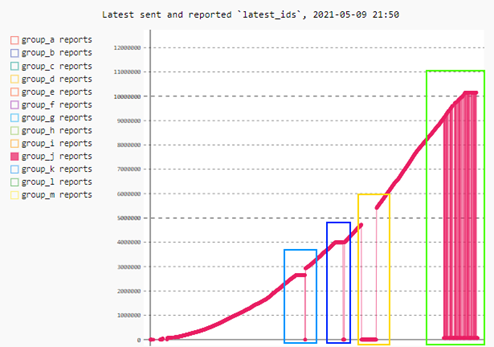
\includegraphics[scale=0.7]{images/downperiodes.png}
    \caption{The graph showing "latest", a int which is updated for each completed job sent from the simulator }
\end{figure}
 
All these different down periods had different solutions, and we have decided to discuss the two down periods we learned the most from, the first down period and the second one. The first down period was due to a crash with our database software (PostgreSQL), and in the second down period it was due to something wrong with the simulator and not on our part. Although logging helped us out in the last down period, we realized to late that the system was down, which resulted in us sometimes being in conflict in what we had agreed to in the SLA. The major lesson learned from the two down periods, was that we should have implemented some sort of alerting sent to all the team members. This was something we started to implement in Kibana, however, due to short time, we did not have the possibility to add this.

\subsubsection{DevOps way of working}

Throughout the project, we as a group have kept the “three ways” characterizing DevOps in mind; flow, feedback and continual learning and experimentation (REFERENCE TO THE DEVOPS HANDBOOK). As deployment have not been a part of our former courses, the principles of flow do not deem so much relevant comparison as the other principles.

One of the main differences from other group work is clearly centered around the feedback principle. In earlier projects, we developed tests as a part of the development, but they were rarely executed. This resulted in hours of development, where the newly developed code was not tested. Therefore, we often had to scrap code and rewrite it. During this project, after the setup of our pipelines, we have been able continuously test our project. We have also used tools such as Sonarcloud and CodeQL. This has led us to not only develop better code, but also ensured that the code was functional and “safe” before it was deployed. This one of the aspects the DevOps way of working impacted our work the most, as it was a huge improvement from how we formerly have been developing.